\chapter{Analisi vettoriale}
In questo capitolo studieremo come e quando è possibile estendere il teorema fondamentale del calcolo integrale, visto in uno dei precedenti capitoli, in più dimensioni, ovvero quando possiamo passare dall'integrazione di un insieme all'integrazione sulla sua frontiera.
Vedremo i principali risultati che si applicano all'analisi vettoriale in $\R^2$ e $\R^3$, in particolare i teoremi della divergenza (Gauss, Ostrogradskij) e del rotore (Green, Stokes).
Per cominciare, vediamo le definizioni degli integrali su linee e superfici in $\R^3$.

\section{Integrali di linea}
Abbiamo già incontrato le curve, anche se solo in $\R^2$, trattando le funzioni implicite.
Vediamone una definizione più generale.
Una \emph{curva} è una funzione $\vphi\colon [a,b]\to\R^n$: diciamo che è regolare se $\vphi\in\cont[1]{[a,b]}$, è iniettiva su $(a,b)$ e $\vphi'(t)\ne\vec 0$ per ogni $t\in(a,b)$.
Spesso è detta curva anche la sua immagine, anche chiamata \emph{sostegno}, $\vphi(I)$, mentre $\vphi$ è detta \emph{parametrizzazione}.

\begin{definizione} \label{d:lunghezza-curva}
	Data una curva $\vphi\colon[a,b]\to\R^n$, definiamo la sua lunghezza $\ell(\vphi)$ come
	\begin{equation}
		\ell(\vphi)=\sup\bigg\{\sum_{i=1}^n\norm{\vphi(t_i)-\vphi(t_{i-1})},\ n\in\N\text{ e }a=t_0<t_1<\cdots<t_n=b\bigg\}
		\label{eq:lunghezza-curva}
	\end{equation}
	dove l'estremo superiore è preso tra tutte le possibili partizioni dell'intervallo $[a,b]$.
	La curva è detta \emph{rettificabile} se $\ell(\vphi)<+\infty$.
\end{definizione}

Definiamo infine la misura infinitesima (o elementare) di una curva come
\begin{equation}
	\dd s\defeq\norm[\bigg]{\drv{\vphi}{t}(t)}\,\dd t
	\label{eq:misura-curva}
\end{equation}
dove $\vphi$ è la sua parametrizzazione.
Con questa definizione, otteniamo la lunghezza della curva parametrizzata da $\vphi$ tramite l'integrale
\begin{equation}
	\ell(\vphi)=\int_\phi\,\dd s=\int_a^b\norm[\bigg]{\drv{\vphi}{t}(t)}\,\dd t
\end{equation}
dove $\phi=\vphi([a,b])$ è l'immagine della curva.
L'integrale di linea di una funzione scalare $f$ definita da $\phi$ a valori in $\R$ è definito come
\begin{equation}
	\int_\phi f\,\dd s=\int_a^b(f\circ\vphi)(t)\norm[\bigg]{\drv{\vphi}{t}(t)}\,\dd t.
\end{equation}
Notiamo che $f\circ\vphi$ è una funzione da $[a,b]$ a $\R$ quindi l'integrale risultante si interpreta senza problemi come un integrale di Lebesgue.

Nel caso in cui una curva regolare sia il grafico di una funzione $\vec f\colon[a,b]\to\R^{n-1}$ di classe $\cont[1]{[a,b]}$, allora la parametrizzazione $\vphi\colon[a,b]\to\R^n$ si scrive facilmente come $\vphi(t)=\big(t,\vec f(t)\big)$, e la misura infinitesima diventa
\begin{equation}
	\dd s=\sqrt{1+\norm{\vec f'(t)}^2}\,\dd t.
\end{equation}

\section{Integrali di superficie}
Innanzitutto, una superficie in $\R^3$ è una funzione $\vphi\colon D\to\R^3$, dove $D$ è un insieme di $\R^2$.\footnote{Anche qui, il termine \emph{superficie} talvolta indica l'immagine della funzione e non la funzione stessa.}
\begin{definizione} \label{d:superficie-regolare}
	Una \emph{superficie regolare} in $\R^3$ è una funzione $\vphi\colon D\to\R^3$ dove $D$ è un insieme connesso di $\R^2$, $\vphi\in\cont[1]{D}$, è iniettiva in $\interior{D}$ e il rango della jacobiana $\jac\vphi$ è massimo in ogni punto di $\interior{D}$.
\end{definizione}
La condizione sul rango della jacobiana è del tutto analoga a quanto già visto per le linee: in tal caso, la jacobiana è composta da una sola colonna, e il rango di una matrice con una sola colonna è 1 (il massimo) se essa è linearmente indipendente, ossia se non è nulla.

\paragraph{Prodotto vettoriale}
Prima di introdurre la misura infinitesima delle superfici, rivediamo le proprietà del prodotto vettoriale.
Dati $\vec u,\vec v\in\R^3$, il prodotto vettoriale tra di essi è il vettore
\begin{equation}
	\vec u\times\vec v=
	\begin{vmatrix}
		u_2& v_2\\u_3&v_3
	\end{vmatrix}\vec e_1+
	\begin{vmatrix}
		u_3&v_3\\u_1&v_1
	\end{vmatrix}\vec e_2+
	\begin{vmatrix}
		u_1&v_1\\u_2&v_2
	\end{vmatrix}\vec e_3
	\label{eq:prodotto-vettoriale}
\end{equation}
dove $\{\vec e_1,\vec e_2,\vec e_3\}$ è la base canonica di $\R^3$.
Notiamo che i tre determinanti sono i minori della matrice ottenuta affiancando $\vec u$ e $\vec v$: in particolare, il coefficiente dell'$i$-esimo elemento della base è il minore di tale matrice eliminando la $i$-esima riga.
Possiamo quindi scrivere in forma più compatta, con un abuso di notazione, una formula mnemonica per calcolare il prodotto vettoriale tramite il falso determinante
\begin{equation*}
	\vec u\times\vec v=
	\begin{vmatrix}
		\vec e_1& u_1& v_1\\
		\vec e_2& u_2& v_2\\
		\vec e_3& u_3& v_3
	\end{vmatrix}.
\end{equation*}
Il prodotto vettoriale gode delle seguenti proprietà, facilmente dimostrabili con le proprietà dei determinanti:
\begin{itemize}
	\item è lineare nelle due variabili: $(a\vec v)\times(b\vec u)=ab(\vec v\times\vec u)$, e $(a\vec v+b\vec u)\times\vec w=a\vec v\times\vec w+b\vec u\times\vec w$;
	\item è nullo se i due vettori sono linearmente dipendenti;
	\item se $\vec v\times\vec w\neq\vec 0$, allora $\vec v\times\vec w\perp\gen{\{\vec v,\vec w\}}$, ossia il prodotto vettoriale è ortogonale al piano individuato dai due vettori, inoltre $\{\vec v,\vec w,\vec v\times\vec w\}$ è una base destrorsa di $\R^3$;
	\item $\vec e_1\times\vec e_2=\vec e_3$, $\vec e_2\times\vec e_3=\vec e_1$ e $\vec e_3\times\vec e_1=\vec e_2$ (permutazioni cicliche);
	\item $\norm{\vec v\times\vec u}=\norm{\vec v}\norm{\vec u}\sin\alpha$, dove $\alpha\in[0,\pi]$ è l'angolo compreso tra i due vettori nel piano, cioè
		\begin{equation}
			\norm{\vec v\times\vec u}=\norm{\vec v}\norm{\vec u}\sin\bigg(\!\arccos\frac{\inner{\vec v}{\vec u}}{\norm{\vec v}\norm{\vec u}}\bigg).
		\end{equation}
	\item il prodotto è indipendente dalla scelta del sistema di coordinate.
\end{itemize}

Con questo possiamo caratterizzare la misura delle superfici.
Se $\vphi\colon D\to\R^3$ è la parametrizzazione scelta per la superficie, la sua misura infinitesima è definita da
\begin{equation}
	\dd\sigma\defeq\norm[\bigg]{\drp{\vphi}{u}(u,v)\times\drp{\vphi}{v}(u,v)}\,\dd u\dd v
	\label{eq:misura-superficie}
\end{equation}
dove abbiamo chiamato $\drp{\vphi}{u}$ e $\drp{\vphi}{v}$ le due colonne che affiancate formano $\jac\vphi$ (sono rispettivamente la colonna delle derivate rispetto alle due variabili $u$ e $v$).
Notiamo che la regolarità della superficie implica che $\dd\sigma\ne 0$ $\forall(u,v)\in D$.

Possiamo vedere una motivazione di questa definizione con l'esempio seguente.
Prendiamo una parametrizzazione $\vphi$ lineare: la sua matrice jacobiana è costante, e può anche essere vista come la matrice associata all'applicazione lineare che è $\vphi$: moltiplicando un vettore del dominio di $\vphi$ per $\jac{\vphi}$ otteniamo proprio l'immagine di tale vettore attraverso la funzione.
Prendiamo il rettangolo $T$ esteso dai vettori $a\vec e_1$ e $b\vec e_2$ in $\R^2$, e sia $P$ la sua immagine attraverso $\vphi$.
Ovviamente $\mu(T)=\abs{ab}$.
Le immagini dei due vettori che individuano $T$ sono $a\drp{\vphi}{x}$ e $b\drp{\vphi}{y}$, quindi abbiamo
\begin{equation*}
	\mu(P)=\norm[\bigg]{a\drp{\vphi}{x}\times b\drp{\vphi}{y}}=\abs{ab}\norm[\bigg]{\drp{\vphi}{x}\times\drp{\vphi}{y}}=\mu(T)\norm[\bigg]{\drp{\vphi}{x}\times\drp{\vphi}{y}}.
\end{equation*}
dato che il prodotto vettoriale $\vec v\times\vec w$ misura l'area del parallalogramma delimitato da $\vec v$ e $\vec w$.
Nella definizione della misura di superficie, dunque, è come se individuassimo un parallelogramma tangente alla superficie nel punto $(u,v)$ individuato dalle due colonne della matrice jacobiana, e ne calcolassimo l'area, ottenendo la \eqref{eq:misura-superficie}.
Il processo è simile alla definizione della misura infinitesima \eqref{eq:misura-curva} di una linea.

L'area della superficie $S=\vphi(D)$ si calcola dunque come
\begin{equation}
	\int_S\dd\sigma=\int_D\norm[\bigg]{\drp{\vphi}{u}(u,v)\times\drp{\vphi}{v}(u,v)}\,\dd u\dd v
\end{equation}
dove $\vphi\colon D\to\R^3$ è la sua parametrizzazione regolare; l'integrale di superficie di una funzione $f\colon S\to\R$ è
\begin{equation}
	\int_Sf\,\dd\sigma=\int_D(f\circ\vphi)(u,v)\norm[\bigg]{\drp{\vphi}{u}(u,v)\times\drp{\vphi}{v}(u,v)}\,\dd u\dd v.
\end{equation}
Anche in questo caso $f\circ\vphi\colon D\to\R$ quindi troviamo un integrale di Lebesgue.

Se una superficie regolare è il grafico di una funzione $g\colon D\subseteq\R^2\to\R$ di classe $\cont[1]{D}$ (si dice in questo caso che è una \emph{superficie cartesiana}), possiamo scegliere la parametrizzazione $\vphi\colon D\to\R^3$ della forma $\vphi(u,v)=\big(u,v,g(u,v)\big)$: la matrice jacobiana è
\begin{equation}
	\begin{bmatrix}
		1&0\\
		0&1\\
		\drp{g}{u}&\drp{g}{v}
	\end{bmatrix}
\end{equation}
da cui
\begin{equation}
	\begin{split}
		\drp{\vphi}{u}\times\drp{\vphi}{v}&=
		\begin{vmatrix}
			0&1\\
			\drp{g}{u}&\drp{g}{v}
		\end{vmatrix}
		\vec e_1+
		\begin{vmatrix}
			\drp{g}{u}&\drp{g}{v}\\
			1&0
		\end{vmatrix}
		\vec e_2+\
		\begin{vmatrix}
			1&0\\
			0&1
		\end{vmatrix}
		\vec e_3=\\
		&=-\drp{g}{u}\vec e_1-\drp{g}{v}\vec e_2+\vec e_3
	\end{split}
	\label{eq:versore-normale-superficie-cartesiana}
\end{equation}
da cui otteniamo la misura infinitesima
\begin{equation}
	\dd\sigma=\sqrt{1+\norm{\grad g(u,v)}^2}\,\dd u\dd v.
\end{equation}

\section{Formule di Gauss-Green}
Cominciamo prima dagli integrali in due dimensioni, per poi introdurre gli integrali di superficie e passare anche a quelli in tre dimensioni.
Per studiare questi teoremi dobbiamo innanzitutto introdurre nuove definizioni per gli insiemi, come quelle di \emph{dominio} e di \emph{orientazione}.
\begin{definizione} \label{d:dominio}
	Un insieme $D\subseteq\R^2$ chiuso si dice \emph{dominio} se è la chiusura di un insieme aperto; si dice inoltre \emph{connesso} se l'aperto di cui è chiusura è connesso.
\end{definizione}
\begin{definizione} \label{d:dominio-norm-reg}
	Un dominio si dice \emph{normale} rispetto alla variabile $x$ se, dato un intervallo $[a,b]$ e due funzioni $f,g\colon[a,b]\to\R$ continue, tali che $f(x)\leq g(x)$ $\forall x\in[a,b]$, esso è della forma $\{(x,y)\in[a,b]\times\R\colon f(x)\leq y\leq g(x)\}$; si definisce in modo analogo per la variabile $y$.
	Si dice \emph{normale} e \emph{regolare} se le funzioni $f$ e $g$ sono di $\cont[1]{[a,b]}$ e se $f(x)<g(x) \forall x\in(a,b)$.
\end{definizione}
\begin{definizione} \label{d:dominio-regolare}
	Un insieme è un \emph{dominio regolare} se è l'unione di un numero finito di domini $D_i$ normali e regolari (rispetto a x oppure a y) separati, ossia $\interior{D_j}\cap\interior{D_k}=\emptyset$ per ogni $j\neq k$.
\end{definizione}
Ogni dominio, essendo chiuso e limitato, è chiaramente anche compatto.

Prendiamo ora la parametrizzazione $\vphi$ di una curva, che sia regolare e definita da $[a,b]$ in $\R^2$: essa è differenziabile in ogni suo punto, dunque esiste il vettore $\vphi'$ per ogni $t\in[a,b]$.
Normalizzando questo vettore otteniamo un versore che indica la direzione tangente alla curva in ogni punto: definiamo dunque il \emph{versore tangente} alla curva $\vphi$ come la funzione $\vphi'/\norm{\vphi'}$, anch'essa da $[a,b]$ a $\R^2$.
A questo punto possiamo definire il \emph{versore normale}, che indicheremo spesso con $\vnu$, come il vettore ottenuto ruotando il versore tangente di $-\pi/2$, ossia
\begin{equation*}
	\vnu(t)=\frac1{\norm{\vphi'(t)}}
	\begin{bmatrix}
		0&1\\-1&0
	\end{bmatrix}
	\begin{bmatrix}
		\phi'_1(t)\\\phi'_2(t)
	\end{bmatrix}
	=\frac1{\norm{\vphi'(t)}}
	\begin{bmatrix}
		\phi'_2(t)\\-\phi'_1(t)
	\end{bmatrix}
\end{equation*}
Chiaramente i due versori sono ortogonali per ogni $t\in[a,b]$.
Se $D$ è un dominio regolare, si può dimostrare che $\boundary D$ è l'unione finita di sostegni di curve regolari a tratti: allora possiamo affermare l'esistenza di un versore tangente e normale alla frontiera di un dominio regolare, tranne al più in un numero finito di punti.

Questo ci porta al problema di trovare un'orientazione delle curve, e più precisamente del bordo di un dominio.
Diremo che la frontiera è orientata in senso \emph{positivo} (e scriveremo $+\boundary D$) se il versore normale ``punta'' all'esterno del dominio (come, ad esempio, nella figura \ref{fig:versore-tangente-normale}).
Questo indica anche il verso di percorrenza della frontiera: percorrendola in senso positivo il dominio si troverà sempre alla sinistra del versore tangente.
\begin{figure}
	\tikzsetnextfilename{versore-tangente-normale}
	\centering
	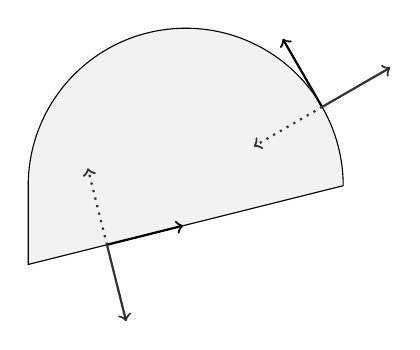
\begin{tikzpicture}
		\draw[fill=black!5!white] (-2,0) -- (-2,-1) -- (2,0) arc (0:180:2);
		% Considero la curva orientata in senso antiorario

		% L'arco è parametrizzato da f(t)=(2*cos(t), 2*sin(t)), t in [0,pi]
		\coordinate (t1) at (1.732,1); % t=pi/6
		\draw[->,thick,black] (t1) -- ++(-.5,.866); % Versore tangente
		\draw[->,thick,black!80!white] (t1) -- ++(.866,.5); % Versore normale uscente
		\draw[->,thick,black!80!white,dotted] (t1) -- ++(-.866,-.5); % Versore normale entrante

		% La retta in basso è parametrizzata da f(t)=(-2+4*t, -1+t), t in [0,1]
		\coordinate (t2) at (-1,-.75); % t=1/4
		\draw[->,thick,black] (t2) -- ++(0.97,.243); % Versore tangente
		\draw[->,thick,black!80!white] (t2) -- ++(.243,.-0.97); % Versore normale uscente
		\draw[->,thick,black!80!white,dotted] (t2) -- ++(-.243,0.97); % Versore normale entrante
	\end{tikzpicture}
	\caption{I versori tangenti e normali al bordo di un dominio regolare di $\R^2$.
		Tale bordo è orientato in senso positivo se è percorso in senso antiorario: in questo modo il versore normale (con tratto continuo) è uscente, e il versore tangente è come indicato.
	L'orientazione in senso negativo dà invece il versore normale entrante (con tratto punteggiato) e il versore tangente opposto.}
	\label{fig:versore-tangente-normale}
\end{figure}


Possiamo dunque dimostrare con gli elementi a disposizione il teorema sviluppato da Gauss e Green.
\begin{teorema}[Gauss-Green] \label{t:gauss-green}
	Sia $D\subseteq\R^2$ un dominio regolare e $f\colon D\to\R$ una funzione in $\cont[1]{D}$.
	Allora valgono
	\begin{gather}
		\int_D\drp{f}{x}(x,y)\,\dd x\,\dd y=\int_{+\boundary D}f(x,y)\,\dd y;
		\label{eq:gauss-green-y}\\
		\int_D\drp{f}{y}(x,y)\,\dd x\,\dd y=-\int_{+\boundary D}f(x,y)\,\dd x.
		\label{eq:gauss-green-x}
	\end{gather}
\end{teorema}
\begin{proof}
	Verrà dimostrata solo la prima legge, la dimostrazione della seconda è del tutto analoga.
	Supponiamo che esista un insieme $U$ aperto tale che $D\subset U$ e che $f\in\cont[1]{U}$.
	Distinguiamo tre casi: (i) $D$ è normale rispetto a $y$, (ii) $D$ è normale rispetto a $x$ e (iii) $D$ è un generico insieme regolare.

	\begin{figure}
	\tikzsetnextfilename{gauss-green-normale-y}
	\centering
	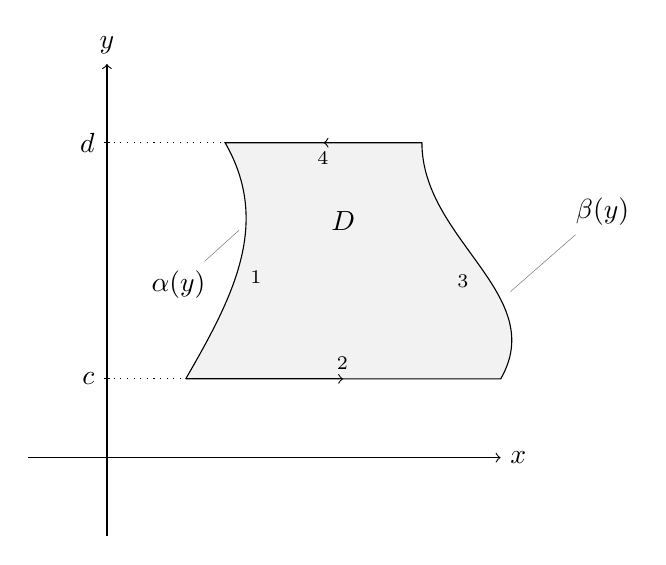
\begin{tikzpicture}
		\draw [black,->] (-1,0) -- (5,0) node[right]{$x$};
		\draw [black,->] (0,-1) -- (0,5) node[above]{$y$};
		\fill [black!5!white] (1,1) -- (5,1) to[out=60,in=270] (4,4) -- (1.5,4) to[out=300,in=60] (1,1);
		% \fill va prima del disegno del contorno, altrimenti si sovrappone a tutto e lo nasconde
		\draw [black] (1,1) to node[auto]{$\vgamma_2$} (5,1)
			to [out=60,in=270] node[auto]{$\vgamma_3$} (4,4)
			to node[auto]{$\vgamma_4$} (1.5,4)
			to [out=300,in=60] node[auto]{$\vgamma_1$} (1,1);
		\draw [dotted] (0,1) -- (1,1);
		\draw [dotted] (0,4) -- (1.5,4);
		\node [pin={[pin distance=5mm]230:{$\alpha(y)$}}] at (1.8,3) {};
		\node [pin={[pin distance=1cm]45:{$\beta(y)$}}] at (5,2) {};
		\node at (3,3) {$D$};
		% Dato che non TikZ non ha un comando per disegnare frecce in mezzo alla linea, mi devo arrangiare.
		% Traccio nuovamente le linee del bordo dell'insieme fino a -- più o meno -- metà, mettendo una freccia sulla
		% punta a queste. Non le disegno sui tratti curvi perche' sarebbe troppo complicato: dovrei spezzare in due anche
		% la linea tracciata prima con \draw (l. 10 e segg.) ma allora l'etichetta con il nome \vgamma del tratto non
		% risulterebbe più centrata.
		\draw [black,->] (1,1) -- (3,1);
		\draw [black,->] (4,4) -- (2.75,4);
		% Queste sono le tacche sull'asse y in corrispondenza delle due linee tratteggiate in y=c e y=d
		\draw (1pt,1) -- (-1pt,1) node[left]{$c$};
		\draw (1pt,4) -- (-1pt,4) node[left]{$d$};
	\end{tikzpicture}
	\caption{Parametrizzazione del contorno di un dominio $D$ come nel punto (i) della dimostrazione del teorema \ref{t:gauss-green} di Gauss-Green.}
	\label{fig:gauss-green-normale-y}
\end{figure}

	(i) Sia $D$ un dominio normale rispetto alla variabile $y$: lo scriviamo allora come $D=\{(x,y)\in\R\times[c,d]\colon \alpha(y)\leq x\leq\beta(y)\}$.
	Suddividiamo il bordo di $D$ nei quattro sottoinsiemi $\gamma_i$ ($i=1,2,3,4$) parametrizzati (come nella figura \ref{fig:gauss-green-normale-y}) con
	\begin{gather*}
		\vgamma_1^-(t)=
		\begin{bmatrix}
			\alpha(t)\\t
		\end{bmatrix}, t\in[c,d],\quad
		\vgamma_2(t)=
		\begin{bmatrix}
			t\\c
		\end{bmatrix}, t\in[\alpha(c),\beta(c)],\\
		\vgamma_3(t)=
		\begin{bmatrix}
			\beta(t)\\t
		\end{bmatrix}, t\in[c,d],\quad 
		\vgamma_4^-(t)=
		\begin{bmatrix}
			t\\d
		\end{bmatrix}, t\in[\alpha(d),\beta(d)].
	\end{gather*}
	Scriviamo $\vgamma_1^-$ e $\vgamma_4^-$ perch\'e la parametrizzazione data è tale che le due curve sono percorse nel senso opposto all'orientazione di $+\boundary D$: nel calcolo dell'integrale dovremo tener conto di questo cambio di segno.
	Dimostriamo che entrambi i membri si possono riportare ad una stessa grandezza: cominciamo dal primo, usando il teorema di Fubini ($f\in\cont[1]{D}$ quindi è anche sommabile), per il quale
	\begin{equation}
		\int_D\drp{f}{x}\,\dd x\,\dd y=\int_c^d\int_{\alpha(y)}^{\beta(y)}\drp{f}{x}\,\dd x\,\dd y=\int_c^df(x,y)\bigg|_{x=\alpha(y)}^{x=\beta(y)}\dd y=\int_c^d\Big[f\big(\beta(y),y\big)-f\big(\alpha(y),y\big)\Big]\,\dd y.
	\end{equation}
	Per il secondo membro, invece, scomponiamo l'integrale della forma differenziale sulle quattro curve ottenendo
	\begin{multline}
		\int_{+\boundary D}f(x,y)\,\dd y=
		-\int_c^d(f\circ\vgamma_1)(t)\gamma'_{1,2}(t)\,\dd t
		+\int_{\alpha(c)}^{\beta(c)}(f\circ\vgamma_2)(t)\gamma'_{2,2}(t)\,\dd t+\\
		+\int_c^d(f\circ\vgamma_3)(t)\gamma'_{3,2}(t)\,\dd t
		-\int_{\alpha(d)}^{\beta(d)}(f\circ\vgamma_4)(t)\gamma'_{4,2}(t),\dd t
	\end{multline}
	dove $\gamma_{k,2}$ è la seconda componente della curva $\vgamma_k$ (per $k=1,2,3,4$).
	Siccome $\gamma'_{1,2}(t)=\gamma'_{3,2}(t)=1$ e $\gamma'_{2,2}(t)=\gamma'_{4,2}(t)=0$ si ha
	\begin{equation}
		\int_{+\boundary D}f(x,y)\,\dd y=\int_c^d\Big[f\big(\beta(t),t\big)-f\big(\alpha(t),t\big)\Big]\,\dd t
	\end{equation}
	che è lo stesso risultato precedente.

	\begin{figure}
	\tikzsetnextfilename{gauss-green-normale-x}
	\centering
	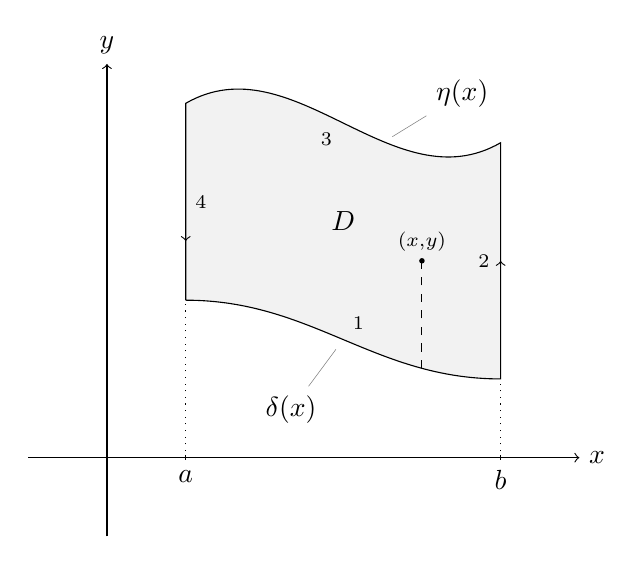
\begin{tikzpicture}
		\draw [black,->] (-1,0) -- (6,0) node[right]{$x$};
		\draw [black,->] (0,-1) -- (0,5) node[above]{$y$};
		\fill [black!5!white] (1,2) to[out=0,in=180] (5,1) -- (5,4) to[out=210,in=30] (1,4.5) -- cycle;
		% \fill va prima del disegno del contorno, altrimenti si sovrappone a tutto e lo nasconde
		\draw [black] (1,2) to[out=0,in=180] node[auto]{$\vgamma_1$} (5,1)
			to node[auto]{$\vgamma_2$} (5,4)
			to[out=210,in=30] node[auto]{$\vgamma_3$} (1,4.5)
			to node[auto]{$\vgamma_4$} (1,2);
		\draw [dotted] (1,0) -- (1,2);
		\draw [dotted] (5,0) -- (5,1);
		\node [pin={[pin distance=5mm]250:{$\delta(x)$}}] at (3,1.5) {};
		\node [pin={[pin distance=5mm]30:{$\eta(x)$}}] at (3.5,4) {};
		\node at (3,3) {$D$};
		% Dato che non TikZ non ha un comando per disegnare frecce in mezzo alla linea, mi devo arrangiare.
		% Traccio nuovamente le linee del bordo dell'insieme fino a -- più o meno -- metà, mettendo una freccia sulla
		% punta a queste. Non le disegno sui tratti curvi perche' sarebbe troppo complicato: dovrei spezzare in due anche
		% la linea tracciata prima con \draw (l. 10 e segg.) ma allora l'etichetta con il nome \vgamma del tratto non
		% risulterebbe più centrata.
		\draw [black,->] (1,4.5) -- (1,2.75); 
		\draw [black,->] (5,1) -- (5,2.5);
		% Queste sono le tacche sull'asse x in corrispondenza delle due linee tratteggiate in x=a e x=b
		\draw (1,1pt) -- (1,-1pt) node[below]{$a$};
		\draw (5,1pt) -- (5,-1pt) node[below]{$b$};
		% Questa è la curva che congiunge l'angolo (a,\delta(a)) in basso a sinistra del bordo con un punto generico nell'insieme.
		% È disegnata per ultima in modo che non sia nascosta da niente.
		% L'angolo di entrata ('in') è una combinazione di fortuna e tanta pazienza: purtroppo non so un modo per calcolarlo
		% automaticamente...
		\draw[black,dashed] (4,1.135) -- (4,2.5) node[above]{$\scriptstyle(x,y)$};
		\fill[black] (4,2.5) circle (1pt);
	\end{tikzpicture}
	\caption{Parametrizzazione del contorno di un dominio $D$ come nel punto (ii) della dimostrazione del teorema \ref{t:gauss-green} di Gauss-Green.}
	\label{fig:gauss-green-normale-x}
\end{figure}

	(ii) Sia ora $D$ normale rispetto a $x$: rappresentiamolo come $\{(x,y)\in[a,b]\times\R\colon\delta(x)\leq y\leq\eta(x)\}$, come in figura \ref{fig:gauss-green-normale-x}.
	Per $(x,y)\in D$, consideriamo la curva $\gamma\subset D$ parametrizzata con la funzione
	\begin{equation*}
		\vgamma(t)=
		\begin{cases}
			\big(t,\delta(t)\big) &t\in[a,x]\\
			(x,t) &t\in[\delta(x),y]
		\end{cases}
	\end{equation*}
	che è regolare a tratti, e collega $\big(a,\delta(a)\big)$ ad un generico punto in $D$.
	Definiamo
	\begin{equation*}
		G(x,y)\defeq\int_{\gamma}f(x,y)\,\dd y:
	\end{equation*}
	risulta, spezzando l'integrale nelle due curve, che
	\begin{equation}
		G(x,y)=\int_a^xf\big(t,\delta(t)\big)\delta'(t)\,\dd t+\int_{\delta(x)}^yf(x,t)\,\dd t.
	\end{equation}
	Calcoliamone le derivate parziali: troviamo
	\begin{equation}
		\drp{G}{x}(x,y)=f\big(x,\delta(x)\big)\delta'(x)+\int_{\delta(x)}^y\drp{f}{x}(x,t)\,\dd t-f\big(x,\delta(x)\big)\delta'(x)=\int_{\delta(x)}^y\drp{f}{x}(x,t)\,\dd t.
	\end{equation}
	La derivata rispetto a $y$ invece è semplicemente $\drp{G}{y}(x,y)=f(x,y)$, dato che il primo dei due integrali addendi non dipende da $y$ e il secondo è una funzione integrale con estremo inferiore costante rispetto a $y$.
	Prendiamo la forma differenziale $\dd G=\drp{G}{x}\,\dd x+\drp{G}{y}\,\dd y$: essa è ovviamente esatta.
	Inoltre $\boundary D$ è chiusa e regolare a tratti, dunque l'integrale di $\dd G$ lungo di essa è nullo: allora
	\begin{equation}
		\int_{+\boundary D}\drp{G}{x}\,\dd x=-\int_{+\boundary D}\drp{G}{y}\,\dd y.
		\label{eq:dim-gauss-green-forma-esatta}
	\end{equation}
	Parametrizziamo il bordo di $D$ con le quattro curve
	\begin{gather*}
		\vgamma_1(t)=
		\begin{bmatrix}
			t\\\delta(t)
		\end{bmatrix}, t\in[a,b],\quad
		\vgamma_2(t)=
		\begin{bmatrix}
			b\\t
		\end{bmatrix}, t\in[\delta(b),\eta(b)],\\
		\vgamma_3^-(t)=
		\begin{bmatrix}
			t\\\eta(t)
		\end{bmatrix}, t\in[a,b],\quad 
		\vgamma_4^-(t)=
		\begin{bmatrix}
			a\\t
		\end{bmatrix}, t\in[\delta(a),\eta(a)].
	\end{gather*}
	Anche qui abbiamo scritto $\vgamma_3^-$ e $\vgamma_4^-$ perché con queste parametrizzazioni le due curve sono percorse nel senso opposto all'orientazione positiva di $\boundary D$, e dovremo cambiare il segno all'integrale.
	Il primo membro di \eqref{eq:dim-gauss-green-forma-esatta}, sostituendo $\drp{G}{x}(x,y)$ trovato prima, vale
	\begin{equation}
		\begin{split}
			\int_{+\boundary D}\drp{G}{x}(x,y)\,\dd x&=\int_{\vgamma_1}\drp{G}{x}(x,y)\,\dd x+\int_{\vgamma_2}\drp{G}{x}(x,y)\,\dd x-\int_{\vgamma_3}\drp{G}{x}(x,y)\,\dd x-\int_{\vgamma_4}\drp{G}{x}(x,y)\,\dd x=\\
			&=\int_a^b\drp{G}{x}\big(s,\delta(s)\big)\,\dd s-\int_a^b\drp{G}{x}\big(s,\eta(s)\big)\,\dd s=\\
			&=\int_a^b\int_{\delta(s)}^{\delta(s)}\drp{f}{x}(s,t)\,\dd t\,\dd s-\int_a^b\int_{\delta(s)}^{\eta(s)}\drp{f}{x}(s,t)\,\dd t\,\dd s=\\
			&=-\int_a^b\int_{\delta(s)}^{\eta(s)}\drp{f}{x}(s,t)\,\dd t\,\dd s.
		\end{split}
	\end{equation}
	Sostituendo poi $\drp{G}{y}(x,y)=f(x,y)$ nella \eqref{eq:dim-gauss-green-forma-esatta} otteniamo\footnote{La variabile $s$ è muta perché è una delle variabili di integrazione, quindi possiamo senza alcun problema porre $x=s$ cambiandone il nome.}
	\begin{equation}
		-\int_a^b\int_{\delta(x)}^{\eta(x)}\drp{f}{x}(x,t)\,\dd t\,\dd x=-\int_{+\boundary D}f(x,y)\,\dd y
	\end{equation}
	e applicando il teorema di Fubini ``al contrario'', cioè passando all'integrale in $D$, troviamo
	\begin{equation}
		\int_D\drp{f}{x}(x,y)\,\dd x\,\dd y=\int_{+\boundary D}f(x,y)\,\dd y.
	\end{equation}

	(iii) Se infine $D$ è un dominio regolare, ma non è normale rispetto ad una delle due variabili, possiamo comunque scomporlo in un insieme di domini normali $\{D_i\}_{i\in I}$ separati.
	Per ciascuno di essi vale quanto detto precedentemente, perciò
	\begin{equation}
		\int_D\drp{f}{x}(x,y)\,\dd x\,\dd y=\sum_{i\in I}\int_{D_i}\drp{f}{x}(x,y)\,\dd x\,\dd y=\sum_{i\in I}\int_{+\boundary D_i}f\,\dd y.
	\end{equation}
	Poich\'e le frontiere dei vari $D_i$ sono in comune, in ciascun addendo di quest'ultima somma ciascuna porzione di frontiera che si trova tra due $D_i$ viene percorsa, integrando, una volta in un senso e una volta nell'altro.
	Chiaramente ciascuna delle due volte la funzione integranda è la stessa, quindi i due integrali hanno segno opposto e si annullano.
	Rimangono nel conto quindi solo le parti delle frontiere che sono esterni, ossia proprio $\boundary D$, quindi
	\begin{equation}
		\sum_{i\in I}\int_{+\boundary D_i}f\,\dd y=\int_{+\boundary D}f\,\dd y.\qedhere
	\end{equation}
\end{proof}

Dato un campo vettoriale $\vec F=(F_1,F_2)\colon U\to\R^2$ di classe $\cont[1]{U}$, definiamo la \emph{divergenza} di $\vec F$ come la funzione $\div\vec F\colon U\to\R$ data da
\begin{equation}
	\div\vec F\defeq\drp{F_1}{x}+\drp{F_2}{y}.
\end{equation}
La divergenza si definisce anche in dimensione qualunque come, dato $\vec F=(F_1,\dots,F_m)$, la funzione
\begin{equation}
	\div\vec F\defeq\sum_{i=1}^m\drp{F_i}{x_i}.
\end{equation}
\begin{teorema} \label{t:divergenza-R2}
	Sia $D\subset\R^2$ un dominio regolare e $\vec F\colon D\to\R^2$ un campo vettoriale di classe $\cont[1]{D}$.
	Se $\vnu(x,y)$ è il versore normale al bordo di $D$ uscente da esso, allora
	\begin{equation}
		\int_D\div\vec F\,\dd x\,\dd y=\int_{\boundary D}\inner{\vec F}{\vnu}\,\dd s.
		\label{eq:divergenza-R2}
	\end{equation}
\end{teorema}
\begin{proof}
	Parametrizziamo $\boundary D$, che è regolare a tratti, con una funzione $\cclass[1]$ a tratti $\vphi(t)=\big(x(t),y(t)\big)$, con $t\in[a,b]$.
	Il versore normale con questa scelta assume quindi la forma
	\begin{equation*}
		\vnu(t)=\frac1{\sqrt{x'^2(t)+y'^2(t)}}
		\begin{bmatrix}
			y'(t)\\-x'(t)
		\end{bmatrix}
	\end{equation*}
	L'integrale curvilineo al secondo membro della \eqref{eq:divergenza-R2} è dunque
	\begin{equation}
		\begin{split}
			\int_{\boundary D}\inner{\vec F}{\vnu}\,\dd s&=\int_a^b\bigg(\frac{(F_1\circ\vphi)(t)y'(t)}{\sqrt{x'^2(t)+y'^2(t)}}-\frac{(F_2\circ\vphi)(t)x'(t)}{\sqrt{x'^2(t)+y'^2(t)}}\bigg)\sqrt{x'^2(t)+y'^2(t)}\,\dd t=\\
			&=\int_a^b\big[(F_1\circ\vphi)(t)y'(t)-(F_2\circ\vphi)(t)x'(t)\big]\,\dd t=\\
			&=\int_{\boundary D}[F_1(x,y)\,\dd y-F_2(x,y)\,\dd x]
		\end{split}
	\end{equation}
	che per il teorema \ref{t:gauss-green} di Gauss-Green è uguale a
	\begin{equation}
		\int_D\drp{F_1}{x}(x,y)\,\dd x\,\dd y+\int_D\drp{F_2}{y}(x,y)\,\dd x\,\dd y=\int_D\div\vec F(x,y)\,\dd x\,\dd y.\qedhere
	\end{equation}
\end{proof}
\begin{teorema} \label{t:rotore-R2}
	Sia $\vec F\colon D\to\R^2$ un campo vettoriale di classe $\cont[1]{D}$ e $D\subset\R^2$ un dominio regolare.
	Allora
	\begin{equation}
		\int_{+\boundary D}\big(F_1(x,y)\,\dd x+F_2(x,y)\,\dd y\big)=\int_D\bigg(\drp{F_2}{x}(x,y)-\drp{F_1}{y}(x,y)\bigg)\,\dd x\,\dd y.
		\label{eq:rotore-R2}
	\end{equation}
\end{teorema}
\begin{proof}
	La dimostrazione è immediata se applichiamo il teorema della divergenza \ref{t:divergenza-R2} al campo $\vec F(x,y)=\big(F_2(x,y),-F_1(x,y)\big)$, per il quale
	\begin{equation}
		\int_{+\boundary D}\inner{\vec F}{\vnu}\,\dd s=\int_{+\boundary D}(F_2(x,y)\,\dd y+F_1(x,y)\,\dd x)=\int_D\drp{F_2}{x}(x,y)\,\dd x\,\dd y-\int_D\drp{F_1}{y}(x,y)\,\dd x\,\dd y
	\end{equation}
	da cui la tesi.
\end{proof}
Grazie a questi teoremi appena dimostrati possiamo portare in più dimensioni la formula di integrazione per parti: si ha, dati $f,g\colon D\to\R$ e $D\subset\R^2$ dominio regolare,
\begin{gather}
	\int_D f(x,y)\drp{g}{x}(x,y)\,\dd x\,\dd y=\int_{+\boundary D}f(x,y)g(x,y)\,\dd y-\int_D\drp{f}{x}(x,y)g(x,y)\,\dd x\,\dd y;\\
	\int_D f(x,y)\drp{g}{y}(x,y)\,\dd x\,\dd y=-\int_{+\boundary D}f(x,y)g(x,y)\,\dd x-\int_D\drp{f}{y}(x,y)g(x,y)\,\dd x\,\dd y.
\end{gather}
Per dimostrarlo è sufficiente applicare il teorema di Gauss-Green \ref{t:gauss-green} alla funzione $fg$.

Dato un versore $\vec w$ di $\R^2$, possiamo anche dare una formulazione del \ref{t:gauss-green} per le derivate direzionali: assumendo sempre $D$ dominio regolare,
\begin{equation}
	\int_DD_{\vec w}f\,\dd x\,\dd y=\int_{\boundary D}f\inner{\vec w}{\vnu}\,\dd s.
\end{equation}
Infatti, applicando il teorema della divergenza \ref{t:divergenza-R2} al campo $f\vec w=(fw_1,fw_2)$, si ottiene
\begin{equation}
	\begin{split}
		\int_D\div(f\vec w)\,\dd x\,\dd y&=\int_D\bigg[\drp{fw_1}{x}(x,y)+\drp{fw_2}{y}(x,y)\bigg]\,\dd x\,\dd y=\\
		&=\int_D\bigg[w_1\drp{f}{x}(x,y)+w_2\drp{f}{y}(x,y)\bigg]\,\dd x\,\dd y=\\
		&=\int_D\inner{\vec w}{\grad f}\,\dd x\,\dd y=\int_DD_{\vec w}f(x,y)\,\dd x\,\dd y
	\end{split}
\end{equation}
ma allo stesso tempo
\begin{equation}
	\int_D\div(f\vec w)\,\dd x\,\dd y=\int_{\boundary D}\inner{f\vec w}{\vnu}\,\dd s=\int_{\boundary D}f\inner{\vec w}{\vnu}\,\dd s.
\end{equation}

Un'ultima applicazione di questi risultati è il calcolo dell'area di $D$: notiamo che in $\int_D\dd x\dd y$ possiamo prendere l'integranda come derivata parziale di $f(x,y)=x$ rispetto a $x$ (che quindi vale 1), perciò per il teorema di Gauss-Green \ref{t:gauss-green} abbiamo
\begin{equation}
	\mu(D)=\int_D\dd x\,\dd y=\int_{+\boundary D}x\,\dd y\text{ o anche }-\int_{+\boundary D}y\,\dd x.
\end{equation}
Possiamo quindi prendere una combinazione arbitraria delle due, in cui presi $\alpha$ e $\beta$ tali che $\alpha+\beta=1$ si ha
\begin{equation}
	\int_{+\boundary D}(\alpha x\,\dd y-\beta y\,\dd x)=(\alpha+\beta)\int_D\dd x\,\dd y=\int_D\dd x\,\dd y=\mu(D).
\end{equation}

\section{Teorema della divergenza e del rotore in $\R^3$}
Cominciamo adattando quanto detto sui domini e l'orientazione di curve anche a insiemi in $\R^3$.
\begin{definizione} \label{d:dominio-R3}
	Un insieme $D\subset\R^3$ si dice:
	\begin{itemize}
		\item \emph{dominio normale} rispetto alla coppia di variabili $x,y$ se si può scrivere come $\{(x,y,z)\in\R^3\colon(x,y)\in E, \alpha(x,y)\leq z\leq\beta(x,y)\}$, dove $E\subset\R^2$ è un dominio regolare, $\alpha,\beta\colon E\to\R$ sono continue e $\alpha(x,y)\leq\beta(x,y)\forall(x,y)\in E$;
		\item \emph{dominio normale e regolare} rispetto alla coppia di variabili $x,y$ se ha le caratteristiche di un dominio normale ma le funzioni $\alpha,\beta\colon E\to\R$ sono di classe $\cont[1]{E}$ e $\alpha(x,y)<\beta(x,y)\forall(x,y)\in E$;
		\item \emph{dominio regolare} se è unione di un numero finito di domini $\{D_i\}_{i=1}^n$, $n\in\N$, ciascuno normale rispetto ad una coppia di variabili (non necessariamente la stessa per tutti), e tali per cui $\interior{D_i}\cap\interior{D_j}=\emptyset$ per $i\neq j$.
	\end{itemize}
\end{definizione}
\begin{osservazione}
	Se $T\subset\R^3$ è un dominio regolare, allora è connesso e compatto, dunque la sua frontiera ha misura nulla.
	Inoltre esiste un numero finito di superfici regolari $\{S_i\}_{i=1}^n$, $n\in\N$, ciascuna parametrizzabile con $\vphi_i\colon D_i\to\R^3$ per $i=1,\dots,n$ (tali quindi che $\vphi_i(D_i)=S_i$), per le quali
	\begin{equation*}
		\boundary T=\bigcup_{i=1}^n\vphi_i(D_i)
	\end{equation*}
	con $\vphi_i(\interior{D_i})\cap\vphi_j(\interior{D_j})=\emptyset$ per $i\neq j$.
\end{osservazione}
D'ora in poi indicheremo sempre con $D$ un dominio regolare di questo tipo.
Possiamo estendere il concetto di integrale di superficie anche a queste frontiere, dato che sono unione numerabile di insiemi disgiunti, a meno di insiemi di misura nulla: infatti l'intersezione di due superfici di cui è composta la frontiera è al più una curva, che ha misura (superficiale) nulla, quindi non influisce sull'integrale.
Se le superfici hanno in comune solo la frontiera, allora\footnote{
	La frontiera di queste superfici è da intendersi nella topologia indotta da $\R^3$ su di esse: se la superficie regolare $S$ è immersa in $\R^3$ infatti $\boundary S=S$.
}
\begin{equation*}
	\int_{\boundary T}f\,\dd\sigma=\sum_{i=1}^n\int_{S_i}f\,\dd\sigma
\end{equation*}
usando la notazione della predecente osservazione.

Prendiamo ora la parametrizzazione $\vphi\colon D\subset\R^2\to\R^3$ di una superficie regolare $S$ immersa in $\R^3$, cioè tale per cui $\vphi(D)=S$: definiamo l'insieme $S_\circ\defeq\vphi(\interior{D})$.
Esso è tale che la restrizione della parametrizzazione $\vphi|_{\interior{D}}\colon\interior{D}\to S_\circ$ è biunivoca.
L'iniettività infatti discende dalla definizione di regolarità della superficie ($\vphi\colon D\to S$ è iniettiva) mentre la suriettività è ovvia per come è stata definita la funzione, poich\'e $S_\circ=\vphi(\interior{D})=\vphi|_{\interior{D}}(\interior{D})$.

Si può vedere che $S_\circ$ non è univoco, ma dipende dalla parametrizzazione.
Prendiamo ad esempio la sfera unitaria $S^2\subset\R^3$, parametrizzata in coordinare polari.
Per coprire tutta $S^2$ dobbiamo prendere le due variabili angolari $(\theta,\phi)\in D=[0,\pi]\times[0,2\pi]$, con
\begin{equation}
	\vphi(\theta,\phi)=
	\begin{pmatrix}
		\sin\theta\cos\phi\\
		\sin\theta\sin\phi\\
		\cos\theta
	\end{pmatrix}.
\end{equation}
L'insieme $S^2_\circ$ in questo caso è l'immagine di $(0,\pi)\times(0,2\pi)$, che è $S^2\setminus\{(x,y,z)\in\R^3\colon y=0,x\ge 0\}$.
Se scegliamo come dominio l'insieme $[0,\pi]\times[\pi,3\pi]$ (la parametrizzazione è \emph{diversa} dalla precedente) troviamo invece $S^2_\circ=S^2\setminus\{(x,y,z)\in\R^3\colon y=0,x\le 0\}$.

\paragraph{Spazio tangente}
Intuitivamente, se abbiamo una curva che corre sulla superficie, un vettore ad essa tangente in un punto è anche tangente alla superficie.
Fissato dunque il punto $\vec x\in S_\circ$, l'insieme dei vettori tangenti a tutte le curve passanti per tale punto forma quello che è chiamato lo \emph{spazio tangente} a $S_\circ$ in $\vec x$.
\begin{definizione} \label{d:spazio-tangente}
	Sia $\vphi\colon D\to S\subset\R^3$ una superficie regolare, e $\vec x$ un punto di $S_\circ$.
	Si definisce \emph{spazio tangente} a $S_\circ$ nel punto $\vec x$ l'insieme, indicato con $T_{\vec x}S_\circ$, formato dai vettori $\vec p\in\R^3$ tali che esiste $\epsilon>0$ e una mappa $\vgamma\colon(-\epsilon,\epsilon)\to\R^3$ di classe $\cclass[1]$ per cui $\vgamma(t)\in S_\circ$ $\forall t\in(-\epsilon,\epsilon)$, $\vgamma(0)=\vec x$, e $\vgamma'(0)=\vec p$.
\end{definizione}
Se $\valpha=(\alpha_1,\alpha_2)\colon I\to\interior{D}$ è una curva regolare, con $I$ intervallo reale (possiamo sceglierlo arbitrariamente in modo che contenga lo zero), allora possiamo prenderne l'immagine attraverso la parametrizzazione ottenendo una curva su $S_\circ$, che è ancora regolare.
Essendo $\interior{D}$ aperto, scelto un punto $(u_0,v_0)$ al suo interno esiste sempre (posto $\valpha(0)=(u_0,v_0)$) un $\epsilon>0$ tale che $\valpha(t)\in\interior{D}$ per ogni $t\in(-\epsilon,\epsilon)$.
Analogamente $(\vphi\circ\valpha)(t)\in S_\circ$ per ogni $t$ in tale intervallo.
Detta $\vec x$ l'immagine di $(u_0,v_0)$ attraverso la parametrizzazione, evidentemente si ha $(\vphi\circ\valpha)(0)=\vec x$.
Allora differenziando la funzione composta otteniamo
\begin{equation}
	(\vphi\circ\valpha)'(0)=\jac\vphi\big(u_0,v_0)\valpha'(0)=\alpha_1'(0)\drp{\vphi}{u}(u_0,v_0)+\alpha_2'(0)\drp{\vphi}{v}(u_0,v_0).
\end{equation}
Si può dimostrare che questa è in effetti la generica espressione di un vettore tangente a una curva di classe $\cclass[1]$ (come richiesto nella definizione \ref{d:spazio-tangente}) passante per il punto $\vec x$: di conseguenza tutti questi vettori tangenti al punto $\vec x$ sono la somma di $\vec x$ e una combinazione lineare delle colonne della matrice jacobiana di $\vphi$.
Riassumendo,
\begin{equation}
	T_{\vec x}S_\circ=\bigg\{\vec x'\in\R^3\colon \vec x'=\vec x+a\drp{\vphi}{u}\big(\vphi^{-1}(\vec x)\big)+b\drp{\vphi}{v}\big(\vphi^{-1}(\vec x)\big),\ \forall a,b\in\R\bigg\}.
	\label{eq:spazio-tangente}
\end{equation}
Tecnicamente $T_{\vec x}S_\circ$ è un \emph{sottospazio affine} di $\R^3$: non è un sottospazio vettoriale, dato che non contiene necessariamente l'origine (possiamo vederlo come un sottospazio vettoriale la cui origine è ``traslata'' in $\vec x$).

\paragraph{Versore normale}
Sapendo ora che lo spazio tangente alla superficie parametrizzata da $\vphi\colon D\to S$ ha come base le due colonne della matrice jacobiana di $\vphi$ (nel senso della \eqref{eq:spazio-tangente}, come sottospazio affine), per ogni $\vec x\in S_\circ$ il vettore $\drp{\vphi}{u}(u,v)\times\drp{\vphi}{v}(u,v)$, con $(u,v)=\vphi^{-1}(\vec x)$, è ortogonale a tale spazio, quindi anche alla superficie in tale punto.
Possiamo dunque definire per ogni $\vec x\in S_\circ$ un versore normale $\vnu(\vec x)$, definito come\footnote{
		Non distinguiamo qui in modo rigoroso la natura dello spazio tangente come sottospazio vettoriale o sottospazio affine.
		Si spera che sia chiaro dal contesto quando i vettori di tale spazio sono spiccati dall'origine oppure dal relativo punto sulla superficie: ad esempio, il versore normale cos\`i definito è da intendersi spiccato dall'origine, cos\`i come i vettori che diremo ortogonali ad esso.
		In parole povere, molti dei vettori relativi agli spazi tangenti sono da interpretarsi ``a meno di una costante'', dove tale costante è il vettore $\vec x$ in cui lo spazio è tangente alla superficie.
	}
\begin{equation}
	\vnu(\vec x)=\frac{\drp{\vphi}{u}(u,v)\times\drp{\vphi}{v}(u,v)}{\norm[\big]{\drp{\vphi}{u}(u,v)\times\drp{\vphi}{v}(u,v)}}.
\end{equation}
Solo per i punti di $S_\circ$ ha senso definire in questo modo il versore normale: se $D$ è chiuso, sulla sua frontiera non ha senso parlare di differenziabilità, perciò le derivate parziali di $\vphi$ sono definite solo per $(u,v)\in\interior{D}$, ossia $\vec x\in S_\circ$.
\begin{osservazione} \label{o:spazio-tangente-superficie-implicita}
	Se una superficie è descritta implicitamente come luogo degli zeri di una funzione $F(x,y,z)$, se le ipotesi del teorema di Dini \ref{t:dini-R3} sono soddisfatte allora possiamo parametrizzarla in un opportuno insieme $A$ con una funzione $\vphi(x,y)=\big(x,y,f(x,y)\big)^T$, come una superficie cartesiana.
	Il versore normale alla superficie è allora
	\begin{equation}
		\vnu(x,y)=-\drp{f}{x}(x,y)\vec e_1-\drp{f}{y}(x,y)\vec e_2+\vec e_3
	\end{equation}
	come già avevamo visto calcolando la misura infinitesima della superficie; un elemento dello spazio tangente in $\vec p_0=\vphi(x_0,y_0)=\big(x_0,y_0,z_0=f(x_0,y_0)\big)^T$ è del tipo $\vec p-\vec p_0$, dove $\vec p=(x,y,z)$, ed è dunque caratterizzato dal fatto di essere ortogonale a tale versore normale, ossia
	\begin{equation}
		0=\inner[\Big]{\vec p-\vec p_0}{\drp{\vphi}{x}(x_0,y_0)\times\drp{\vphi}{y}(x_0,y_0)}=
		-(x-x_0)\drp{f}{x}(x_0,y_0)-(y-y_0)\drp{f}{y}(x_0,y_0)+z-z_0
	\end{equation}
	ma sempre per il teorema di Dini esprimiamo le derivate parziali di $f$ in termini delle derivate parziali di $F$ ottenendo
	\begin{equation}
		0=(x-x_0)\dfrac{\drp{F}{x}(x_0,y_0,z_0)}{\drp{F}{z}(x_0,y_0,z_0)}+(y-y_0)\dfrac{\drp{F}{y}(x_0,y_0,z_0)}{\drp{F}{z}(x_0,y_0,z_0)}+z-z_0
	\end{equation}
	da cui ricaviamo l'equazione dello spazio tangente in $\vec p_0$:
	\begin{equation}
		\drp{F}{x}(\vec p_0)(x-x_0)+\drp{F}{y}(\vec p_0)(y-y_0)+\drp{F}{z}(\vec p_0)(z-z_0)=0
		\label{eq:spazio-tangente-superficie-implicita}
	\end{equation}
	o anche in breve, $\inner{\grad F(\vec p_0)}{\vec p-\vec p_0}=0$.
	Questo mostra tra l'altro che il gradiente di $F$ è ortogonale alla superficie in tale punto.
\end{osservazione}

\begin{definizione} \label{d:superficie-orientabile}
	Sia $S\subset\R^3$ una superficie regolare parametrizzata da $\vphi\colon D\to\R^3$: essa si dice orientabile se il campo del versore normale $\vnu$ si può estendere con continuità da $S_\circ$ a tutta $S$.
\end{definizione}
Prese due superfici regolari $\vphi_1\colon D_1\to\R^3$ e $\vphi_2\colon D_2\to\R^3$, possiamo chiederci, come già visto per le curve, quando sono \emph{equivalenti}; in breve, vogliamo trovare un cambiamento di coordinate $\vtau\colon D_1\to D_2$ che sia di classe $\cclass[1]$.
Anche qui però non ha senso parlare di differenziabilità sulla frontiera di un insieme, quindi è meglio perfezionare la definizione.
Diciamo che le due superfici sono equivalenti se:
\begin{itemize}
	\item esiste una funzione (comunemente, una \emph{riparametrizzazione}) $\vtau\colon E\to\R^2$, con $E$ aperto tale che $D_1\subset E$ e $D_2\subset\vtau(E)$, di classe $\cont[1]{E}$ e tale che $\vtau^{-1}$ sia a sua volta di classe $\cclass[1]$, in altre parole un diffeomorfismo tra $E$ e la sua immagine;\footnote{
		La continuità dell'inversa assicura che anche $\vtau(E)$ è aperto.
	}
	\item hanno la stessa immagine, ossia $\vphi_1(D_1)=\vphi_2(D_2)$. 
\end{itemize}
\begin{figure}
	\tikzsetnextfilename{riparametrizzazione-superfici}
	\centering
	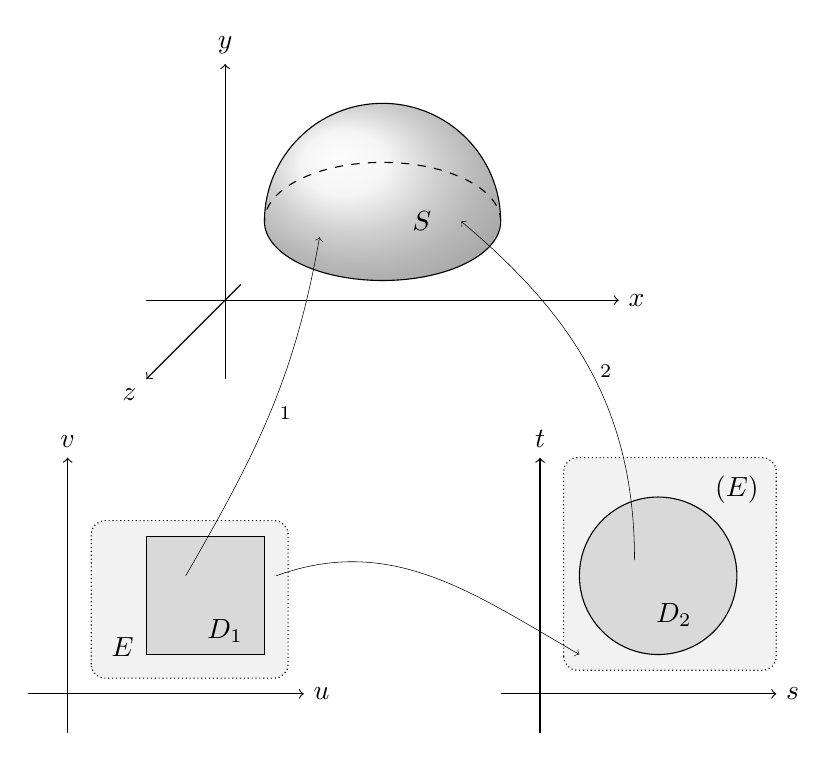
\begin{tikzpicture}
		% Dove possibile ho usato delle coordinate relative alle varie origini dei sistemi di assi
		% che ho disegnato, in modo da facilitare le modifiche.
		% Purtroppo \node e \coordinate ammettono solo coordinate assolute...

		% Piano R^2 per il dominio D_1
		\coordinate (O1) at (0,0);
		\draw [black,->] (O1) +(-.5,0) -- ++(3,0) node[right]{$u$};
		\draw [black,->] (O1) +(0,-.5) -- ++(0,3) node[above]{$v$};

		\draw [fill=black!5!white,densely dotted,rounded corners=5pt] (.3,.2) rectangle +(2.5,2);
		% Disegno un insieme (i.e. E_1) che includa D_1 (il contorno punteggiato dovrebbe
		% suggerire che è un insieme aperto). Dato che va sullo sfondo, lo disegno per primo
		% altrimenti copre D_1.
		\node (E1) at (.7,.6) {$E$};
		\draw [fill=black!15!white,solid] (O1) +(1,.5) rectangle +(2.5,2); % Il dominio D_1
		\node (D1) at (2,.8) {$D_1$};

		% Piano R^2 per il dominio D_2 (traslato di (6,0) rispetto al precedente)
		\coordinate (O2) at (6,0);
		\draw [black,->] (O2) +(-.5,0) -- ++(3,0) node[right]{$s$};
		\draw [black,->] (O2) +(0,-.5) -- ++(0,3) node[above]{$t$};
		
		\draw [fill=black!5!white,densely dotted,rounded corners=5pt] (O2) +(.3,.3) rectangle ++(3,3); % tau(E)
		\node (E2) at (8.5,2.6) {$\vtau(E)$};
		\draw [fill=black!15!white,solid] (O2)+(1.5,1.5) circle (1); % Il dominio D_2
		\node (D2) at (7.7,1) {$D_2$};

		% Spazio R^3 per la superficie (traslato di (2,5) rispetto al piano di D_1)
		\coordinate (O3) at (2,5);
		\draw [black,->] (O3) +(-1,0) -- ++(5,0) node[right]{$x$};
		\draw [black,->] (O3) +(0,-1) -- ++(0,3) node[above]{$y$};
		\draw [black,->] (O3) +(.2,.2) -- ++(-1,-1) node[below left]{$z$};

		\coordinate (C) at (4,6); % Coordinata del centro della "sfera" (relativa a O1)
		\shade[ball color=black!10!white,semitransparent] (C) +(-1.5,0) arc (180:360:1.5 and .75) arc (0:180:1.5);
		% Crea una sfumatura che ricorda la luce riflessa da una sfera (il percorso specificato è il contorno
		% della figura disegnata con i tre archi), come al solito da disegnare prima delle linee di contorno
		\draw[dashed] (C) +(1.5,0) arc (0:180:1.5 and .75); % Semicirconferenza "nascosta" dietro
		\draw (C) +(-1.5,0) arc (180:360:1.5 and .75); % Semicirconferenza "di fronte"
		\draw (C) +(1.5,0) arc (0:180:1.5); % L'arco più grande
		\node (S) at (4.5,6) {$S$};

		% Funzioni tra gli insiemi
		% (Non so bene come usare qui le coordinate relative...)
		\draw [very thin,->] (2.65,1.5) to[out=20,in=150] node[above] {$\vtau$} (6.5,.5);
		\draw [very thin,->] (1.5,1.5) to[out=60,in=260] node[right] {$\vphi_1$} (3.2,5.8);
		\draw [very thin,->] (7.2,1.7) to[out=90,in=320] node[right] {$\vphi_2$} (5,6);
	\end{tikzpicture}
	\caption{Riparametrizzazione di una superficie tramite un diffeomorfismo.}
	\label{fig:riparametrizzazione-superfici}
\end{figure}

L'equivalenza tra le due superfici si indica con $\vphi_1\sim\vphi_2$.
Vediamo come varia il versore normale quando cambiamo la parametrizzazione: usiamo la notazione appena introdotta, con il diffeomorfismo $\vtau=(\tau_1,\tau_2)$ tra l'aperto $E\supset D_1$ e la sua immagine, indicando con $(u,v)$ le coordinate in $D_1$ e con $(s,t)$ quelle in $D_2$ (cosicch\'e $\vtau\colon(u,v)\mapsto(s,t)$); detto $\vnu_1$ il versore normale a $S$ con la parametrizzazione $\vphi_1$ e $\vnu_2$ quello con $\vphi_2$, risulta
\begin{equation}
	\begin{split}
		\drp{\vphi_1}{u}\times\drp{\vphi_1}{v}&=\bigg(\drp{\vphi_2}{s}\drp{\tau_1}{u}+\drp{\vphi_2}{t}\drp{\tau_2}{u}\bigg)\times\bigg(\drp{\vphi_2}{s}\drp{\tau_1}{v}+\drp{\vphi_2}{t}\drp{\tau_2}{v}\bigg)=\\
		&=\drp{\vphi_2}{s}\drp{\tau_1}{u}\times\drp{\vphi_2}{t}\drp{\tau_2}{v}+\drp{\vphi_2}{t}\drp{\tau_2}{u}\times\drp{\vphi_2}{s}\drp{\tau_1}{v}=\\
		&=\drp{\tau_1}{u}\drp{\tau_2}{v}\bigg(\drp{\vphi_2}{s}\times\drp{\vphi_2}{t}\bigg)-\drp{\tau_2}{u}\drp{\tau_1}{v}\bigg(\drp{\vphi_2}{s}\times\drp{\vphi_2}{t}\bigg)=\\
		&=\det(\jac\vtau)\bigg(\drp{\vphi_2}{s}\times\drp{\vphi_2}{t}\bigg)
	\end{split}
\end{equation}
dunque normalizzando si ha
\begin{equation}
	\vnu_1=\sgn\big(\!\det(\jac\vtau)\big)\vnu_2.
	\label{eq:versore-normale-riparametrizzazione}
\end{equation}
Per la continuità del versore normale, il segno della matrice jacobiana può essere quindi o 1 o $-1$ in tutto il dominio, perciò o vale $\vnu_2(\vec x)=\vnu_1(\vec x)$ o vale $\vnu_2(\vec x)=-\vnu_1(\vec x)$ per ogni $\vec x\in S_\circ$.
Indichiamo quindi con $\vphi_1\overset{\circ}{\sim}\vphi_2$ se le due superfici sono anche equiorientate, cioè se il versore normale coincide (ha lo stesso segno).
\begin{esempio} \label{es:versore-normale-sfera}
	Prendiamo una sfera di raggio $R$, centrata nell'origine: è il luogo degli zeri della funzione $F(x,y,z)=x^2+y^2+z^2-R^2$, e prendendo solo l'emisfero per $z>0$ possiamo applicare il teorema di Dini.
	Per quanto visto nell'osservazione \ref{o:spazio-tangente-superficie-implicita}, il versore normale è
	\begin{equation}
		\vnu(x,y,z)=\frac{\grad F(x,y,z)}{\norm{\grad F(x,y,z)}}=\frac1{\sqrt{4x^2+4y^2+4z^2}}(2x,2y,2z)^T=\frac1{R}(x,y,z)^T
	\end{equation}
	quindi punta sempre nella direzione radiale.
	L'estensione di $\vnu$ a tutta la superficie si vede subito sfruttandone la simmetria.
	Essa è evidentemente sempre orientabile, e le due orientazioni possibili sono quella uscente ($\vnu$) o quella entrante ($-\vnu$).
\end{esempio}
\begin{esempio} \label{es:nastro-moebius}
	Il nastro di M\"obius è una superficie non orientabile, data dalla parametrizzazione
	\begin{equation}
		\vphi(u,v)=\bigg(
			\Big(r+\dfrac{v}2\cos\dfrac{u}2\Big)\cos\dfrac{u}2,\
			\Big(r+\dfrac{v}2\cos\dfrac{u}2\Big)\sin\dfrac{u}2,\
			\dfrac{v}2\sin\dfrac{u}2
		\bigg)^T
		\label{eq:nastro-moebius}
	\end{equation}
	per $(u,v)\in[-a,a]\times[0,2\pi]$, con $a,r\in\R$ fissati: essa descrive un nastro di larghezza $a$ il cui punto medio percorre una circonferenza (centrata nell'origine) di raggio $r$.
	Se $a<r$ la superficie non si interseca ed è dunque una superficie regolare.
	\begin{figure}
	\tikzsetnextfilename{nastro-moebius}
	\centering
	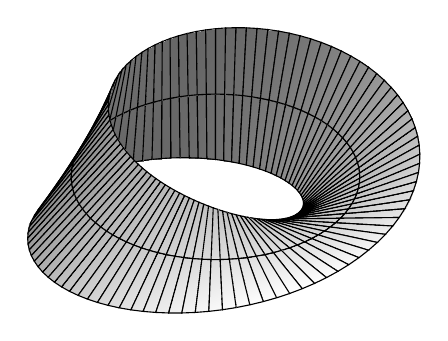
\begin{tikzpicture}
		\begin{axis}[
			trig format plots=rad, % Imposta gli angoli in radianti (dovrebbe esserci un'impostazione globale...) 
			unit vector ratio=1 1 1, % Rapporti tra le lunghezze nelle tre direzioni
			hide axis, % Tengo nascosti gli assi perche' servono a poco in questo caso
			view={70}{35} % {angolo azimutale}{elevazione, attorno all'asse x ruotato}, in gradi/360
			% Con un'elevazione < 30 il nastro appare troppo schiacciato
			% Ho trovato una buona combinazione con un po' di pazienza ;-)
			]
			\addplot3[
				surf,
				faceted color=black,
				shader=faceted interp, % Determina la colorazione della superficie:
				% 'faceted interp' determina il colore di ogni "frammento" della figura
				% con un algoritmo di interpolazione e colora il contorno di ciascuno di essi
				% con il valore assegnato a 'faceted color' precedentemente
				point meta=x, % Per basare la colorazione della superficie sul valore di x
				colormap={bw}{gray(0cm)=(0.4); gray(1cm)=(1)}, % Una colorazione da grigio a bianco
				samples=100,
				samples y=3, % Questo disegna tre righe ``orizzontali'', una in mezzo e due al bordo
				z buffer=sort, % Determina quali parti dell'immagine devono essere disegnate per prime: 'sort'
				% lo decide in modo intelligente, in base alla profondità dei punti
				domain=0:6.284, % x è l'angolo, che va da 0 a poco più di 2pi
				y domain=-1:1 % y è l'altezza del nastro (con questo intervallo è alto 1)
			] (
				{(1+y/2*cos(x/2))*cos(x)},
				{(1+y/2*cos(x/2))*sin(x)},
				{y/2*sin(x/2)}
			);
		\end{axis}
	\end{tikzpicture}
	\caption{Un esempio di nastro di M\"obius, ottenuto dalla \eqref{eq:nastro-moebius} con $r=1$ e $a=1$. Percorrendo la circonferenza al centro del nastro si può notare che fissato localmente un versore normale e prolungandolo per continuità su tutto il nastro, compiendo un giro di $2\pi$ il versore normale risulta orientato nel verso opposto.}
	\label{fig:nastro-moebius}
\end{figure}

	Per semplicità, calcoliamo un vettore normale, senza normalizzarlo, solo nella circonferenza di mezzo, vale a dire per $v=0$: esso vale
	\begin{equation}
		\vnu(u,0)=\bigg(
			\dfrac14\cos\dfrac{u}2\sin u,\
			\dfrac14\sin\dfrac{u}2\sin u,\
			-\dfrac14\cos\dfrac{u}2
		\bigg)^T
		\label{eq:vettore-normale-centro-nastro-mobius}
	\end{equation}
	Vediamo che quando $u$ varia da 0 a $2\pi$ $\vnu$ cambia segno, dato che le funzioni sono periodiche di $4\pi$: ma dalla \eqref{eq:nastro-moebius} è chiaro che $\vphi(0,0)$ e $\vphi(2\pi,0)$ \emph{sono lo stesso punto}, perciò il vettore normale non può essere ben definito su tutta la superficie.
	Chiaramente possiamo avere un vettore normale ben definito per $(u,v)\in(-1,1)\times(0,2\pi)$: il problema si ha quando vogliamo aggiungere il bordo, in cui il vettore normale ``salta'' da una faccia all'altra.\footnote{
		In realtà è sbagliato parlare di ``facce'' del nastro di M\"obius, in quanto (come uno sguardo alla figura può subito far capire) di faccia ce n'è \emph{una sola}.
		Se localmente, in un intorno di un qualsiasi punto (non sul bordo) del nastro, sembra che ci possano essere due facce, questo non può più essere vero globalmente.
	}
\end{esempio}

\begin{definizione} \label{d:superfici-con-bordo}
	Sia $\vphi\colon D\to\R^3$ la parametrizzazione di una superficie $S$ regolare, con $D$ dominio regolare connesso: essa si dice \emph{superficie con bordo} se $\vphi$ è iniettiva su $D$ e se si può individuare un insieme $E\supset D$ aperto e una funzione $\tilde{\vphi}\colon E\to\R^3$, di classe $\cont[1]{E}$, tale che la sua restrizione in $D$ coincida con $\vphi$. Il rango della jacobiana $\jac\vphi$ deve essere massimo $\forall (u,v)\in D$.
\end{definizione}
Per queste superfici definiamo allora $\boundary S\defeq\vphi(\boundary D)$.
Il bordo di $D$, che è un dominio regolare, si può esprimere sempre come unione di curve semplici, regolari a tratti.
Se dunque $\vgamma$ è una parametrizzazione di $+\boundary D$ (cioè tale che il versore normale al bordo di $D$ è uscente), allora componendo la parametrizzazione della superficie, $\vphi$, con essa si ottiene $\vphi\circ\vgamma$ che è una parametrizzazione del bordo di $S$, ed è una curva regolare a tratti in $\R^3$.
In questo caso si scrive $+\boundary S$, e il bordo $\boundary S$ diventa orientato in senso antiorario (e si dice che l'orientazione è indotta da quella di $\boundary D$).

Possiamo dunque concludere con le versioni dei teoremi del rotore e della divergenza per campi vettoriali in $\R^3$, di cui non diamo la dimostrazione.
\begin{teorema}[Gauss-Ostrogradsky] \label{t:divergenza-R3}
	Se $D\subset\R^3$ è un dominio regolare e $\vec F\colon D\to\R^3$ un campo vettoriale $\cont[1]{D}$, allora
	\begin{equation}
		\int_{\boundary D}\inner{\vec F}{\vnu}\,\dd\sigma=\int_D\div\vec F\,\dd x\,\dd y\,\dd z.
		\label{eq:divergenza-R3}
	\end{equation}
	dove $\vnu$ è il versore normale a $\boundary D$ \emph{uscente} da $D$.
\end{teorema}
\begin{corollario}
	Sia $D\subset\R^3$ regolare, $f\colon D\to\R$ una funzione $\cont[1]{D}$, e $\vec w\in\R^3$ un versore.
	Allora
	\begin{equation}
		\int_DD_{\vec w}f\,\dd x\,\dd y\,\dd z=\int_{\boundary D}f\inner{\vec w}{\vnu}\,\dd\sigma.
	\end{equation}
	dove $D_{\vec w}$ indica la derivata lungo la direzione di $\vec w$, e $\vnu$ è il versore normale a $\boundary D$ uscente.
\end{corollario}
\begin{proof}
	Il campo $f\vec w$ è una funzione da $D$ a $\R^3$, e la sua divergenza è $\div(f\vec w)=\sum_{i=1}^3\drp{f}{x_i}w_i=\inner{\vec w}{\grad f}=D_{\vec w}f$: dal teorema precedente
	\begin{equation}
		\int_{\boundary D}\inner{f\vec w}{\vnu}\,\dd\sigma=\int_D\div(f\vec w)\,\dd x\,\dd y\,\dd z=\int_DD_{\vec w}f\,\dd x\,\dd y\,\dd z.\qedhere
	\end{equation}
\end{proof}
Un altro caso particolare, che discende da questo corollario, è la formula di integrazione per parti: sempre in generale con le derivate direzionali, applicandolo alla funzione $\vec F=fg\vec w$ otteniamo
\begin{equation}
	\int_Df(D_{\vec w}g)\,\dd x\,\dd y\,\dd z=\int_{\boundary D}fg\inner{\vec w}{\vnu}\,\dd\sigma-\int_D(D_{\vec w}f)g\,\dd x\,\dd y\,\dd z.
\end{equation}
Sempre con l'ultimo corollario, prendendo invece per $\vec w$ un versore $\vec e_i$ della base canonica risulta
\begin{equation}
	\int_DD_{\vec e_i}f\,\dd x\,\dd y\,\dd z=\int_D\drp{f}{x_i}\,\dd x\,\dd y\,\dd z=\int_{\boundary D}\inner{f\vec e_i}{\vnu}\,\dd\sigma=\int_{\boundary D}f\nu_i\,\dd\sigma.
\end{equation}
Dato un campo vettoriale $\vec F=(F_1,F_2,F_3)\colon U\to\R^3$ di classe $\cont[1]{U}$, definiamo il \emph{rotore} di $\vec F$ come la funzione $\rot\vec F\colon U\to\R^3$ data da
\begin{equation}
	\rot\vec F\defeq\bigg(
		\drp{F_3}{y}-\drp{F_2}{z},
		\drp{F_1}{z}-\drp{F_3}{x},
		\drp{F_2}{x}-\drp{F_1}{y}
		\bigg)^T
\end{equation}
Come per la divergenza, anche al rotore è collegato un teorema omonimo.\footnote{
	Anche il teorema \ref{t:rotore-R2} si potrebbe chiamare ``teorema del rotore'', se volessimo estendere la definizione del rotore alle funzioni in $\R^2$ come $\rot\colon\vec F=(F_1,F_2)\mapsto \partial_1{F_2}-\partial_2F_1$.
}
\begin{teorema}[Kelvin-Stokes] \label{t:rotore-R3}
	Sia $S\subset\R^3$ una superficie regolare con bordo e $\vphi\colon D\to\R^3$ una sua parametrizzazione, con $D\subset\R^2$ dominio regolare.
	Sia inoltre $A$ un aperto di $\R^3$ tale che $S\subset A$, e $\vec F\colon A\to\R^3$ un campo di classe $\cont[1]{A}$.
	Allora
	\begin{equation}
		\int_S\inner{\rot\vec F}{\vnu}\,\dd\sigma=\int_{+\boundary S}\inner{\vec F}{\vec t}\,\dd s
		\label{eq:rotore-R3}
	\end{equation}
	dove $\vec t$ è il versore tangente a $+\boundary S$.
\end{teorema}
